\chapter{Introduction}

During the course of my graduate research, I have worked on two sets of projects. In the first, I developed a set of analytical and numerical tools for studying a certain class of statistical mechanics models. These models potentially have a number of applications, but the application I focused on was topological phases of bosons. In the end I was able to produce numerically tractable models of topological phases in one, two and three dimensions. This series of projects occupied the majority of my time during my degree. 
More recently, I have been working on projects related to the numerical study of the fractional quantum Hall effect. What these two sets of projects have in common is that they are both studies of topological phases of matter. Therefore this thesis begins with a discussion and motivation for the study of topological phases.

\section{Introduction to Topological Phases}

A central concept is condensed matter physics is that of phase transitions, which are locations in parameter space where the free energy is not analytic. From this we can arrive at the definition of a `phase of matter': two states of a material are in different phases if there is path in parameter space which connects them and which does not cross a phase transition. It has long been known that different phases of matter can have different qualitatively different properties. This understanding was put on a firmer footing by Landau\cite{Wen_book}, who pointed out that these qualitatively different properties arise because different phases have different symmetries.  For example, paramagnetic phases have time-reversal symmetriews while ferromagnetic phases break that symmetry. Liquids have translational symmetry while crystals do not. Given a material known to undergo a phase transition, the task of the condensed matter physicist was to determine the symmetry which was breaking across the transition.


%When discussing topology in condensed matter systems, it is helpful to contrast with the situation before the introduction of topology. In that time, it was thought that all phases of matter could be uniquely described by their symmetries.

This understanding was overturned by the discovery of the quantum Hall effect in 1980.\cite{klitzing} In the quantum Hall effect, each Hall plateau corresponds to a different phase of matter (different plateaus cannot be turned into each other without undergoing a phase transition), but all the phases have the same symmetry. What is different between the different phases turns out to be a topological invariant known as the Chern number. We call the Chern number a topological invariant because it is the result of integrating a function (in this case the Berry curvature) over a topologically non-trivial manifold (in this case a torus). An interesting property of topological invariants is that they are independent of the metric of the manifold, they care only about its topology. There such invariants can take exactly the same value everywhere within the same phase. 
%explanation as to why the chern number is topological (from bernevig)

There are many general statements which can be made about symmetry-breaking transitions in condensed matter physics. 
Examples of such general properties include the fact that the breaking of a symmetry can be detected by an order parameter, and that properties at a critical point are determined by  critical exponents independent of the microscopic details of the system. We also know about the point groups, which tell us all the different ways to break spatial symmetries, and that breaking continuous symmetries leads to Goldstone modes. These general facts help us to understand symmetry-breaking transitions.
%Some examples include order parameters, and that they possess 

Since the discovery of phases which are described by topological invariants and not symmetyr breaking, important area of research is to establish similar general principles. Much progress has been made in this direction over the past several years, and in the remainder of this section, I will describe a number of these properties which will be used throughout this work.

The concept of entanglement is crucial to the study of topological phases. Perhaps the simplest system which exhibits entanglement is a pair of spin-1/2 particles which form a spin singlet. Even if the two particles are well separated in space, it is still possible for the state of one to affect the state of the other. A condensed matter system which contains many spin singlets macroscopically far apart would have a lot of entanglement, whereas a system with few, or very close together, singlets would have little entanglement. As early as 1935 it was realized by Einstein\cite{Einstein} that this entanglement leads to highly counterintuitive results, and so it should be no surprise that most of the matter around us has very little entanglement.

With this in mind, we can divide all states of matter into two classes: short-ranged entangled (SRE) and long-ranged entangled (LRE). 
In an SRE phase the entanglement between two spatially separated subsystems decays as exponentially in the separation, while for an LRE system it is either constant or decays as a power law. We will see that long-ranged entangled matter can have a variety of very interesting (and perhaps even useful) properties. Topological phases can have either short- or long-ranged entanglement, and these two cases will be discussed separately.

\subsection{Short-ranged Entangled Topological Phases}

Even in the absence of long-ranged entanglement, topological phases of matter can still have exotic properties. In addition, short-ranged entangled phases are arguably simpler to understand than their long-ranged cousins, and so they are a good place to begin any study of topological phases.

Perhaps the most important events so far in the study of SRE topological phases were the discovery of the quantum spin Hall effect\cite{QSHEreview} and the topological insulator(TI).\cite{KaneHasanRMP,QiZhangRMP}
\footnote{The term `topological insulator' is used in the literature to describe a number of different phases, in this work I will use it exclusively to describe the 3D `strong' TI}
Like the integer quantum Hall effect, these phases have topological invariants, which can be computed by integrating the Berry curvature over the Brillioun zone. Unlike the IQHE, these topological invariants are \emph{only quantized in the presence of time-reversal symmetry}. This means that these topological phases only exist when this symmetry is present. This turns out to be a general property of SRE topological phases:
\footnote{With the exception of chiral phases}
 they become topologically trivial if certain symmetries are broken. These phases are often called `symmetry protected topological phases' (SPTs).

The topological invariant in both the spin Hall effect and the topological insulator is a total derivative. Therefore 
%unlike in the quantum Hall effect 
there is no bulk measurement which can distinguish these phases from topologically trivial phases with the same symmetry. There is however exotic edge physics that takes place on the interface between topological and non-topological matter which can distinguish between the two cases. For example, the quantum spin Hall effect has two counterpropagating edge modes (each carrying opposite spin). This cannot happen in a purely one-dimensional system with time-reversal symmetry.\cite{NN} The topological insulator has a single Dirac cone, which cannot happen in a two-dimensional time-reversal-invariant system. This is another general property of SRE topological systems: they can host edge physics which cannot exist in a system of one lower dimension.

One may also ask what other SRE topological phases are possible, besides the ones given above. Answers to this question take the form of `classification tables', which, given a symmetry and number of dimensions, tell us how many topological phases there are. Classification tables for free fermion systems\cite{KitaevClass,Ludwig} as well as bosons\cite{WenScience,WenPRB,KapustinThorngren} have been produced, which classify many possible cases, though a complete classification is still an area of active research. Such classification tables provide a roadmap in the search for more examples of SRE topological phases.

\subsection{Long-ranged entanglement}
\label{subsec::LRE}

There are three situations in which matter can have long-ranged entanglement. One is at a critical point, where the entanglement decays algebraically in space. If we are interested in accessing long-ranged entanglement experimentally this is not very useful, as critical points require a lot of fine-tuning and are by definition unstable. Another possibility is if the state is gapless (for example, if it has Goldstone modes). The only known way to get a stable, gapped phase with long-ranged entanglement is if the phase is topological. 

Like the SRE topological phases discussed above, LRE topological phases can have exotic physics. Unlike SRE phases, LRE phases to not require symmetry to exist. They also have other exotic properties, in particular \emph{fractionalization}. This means that the gapped quasiparticles in a LRE phase can carry fractions of the quantum numbers (such as charge). Much of the physics of LRE phases was first developed during the study of the fractional quantum Hall effect (FQHE). For example, a filling $\nu=1/3$ FQHE system has quasiparticles carrying $1/3$ charge\cite{Laughlin-PhysRevLett.50.1395}. The spin of the quasiparticles can also become fractionalized. In an SRE system all quasiparticles must be either bosons or fermions, which means that upon interchanging two quasiparticles the phase of the wave function must change by $\pm 1$. In an LRE system quasiparticles (in two dimensions) can be `anyons', and interchanging them can either multiply the wave function by any complex phase\cite{LeinaasMyrheim, Arovas-Schrieffer-Wilczek} (if the anyons are Abelian), or put the system into a different degenerate ground state (for non-Abelian anyons, which will be explained in more detail below). 
From the anyonic statistics of the quasiparticles we can also show that LRE topological phases have a ground state degeneracy when put on a topologically non-trivial surface(e.g.~a torus). This is because the operations of taking a quasiparticle around the different cycles of the torus do not commute.

\section{Tractable Models of Interacting Topological Phases}

	We can see that many general properties of topological phases have been determined. Note that though those properties hold in general, the concepts were first established for specific examples of topological phases, such as the quantum spin Hall effect, topological insulator and fractional quantum Hall effect. To learn about other general properties of topological phases, we may need to study other specific examples of topological phases. In particular, we may be interested in topological phases which have strong interactions, unlike many of the familiar topological phases, such as the integer quantum Hall effect and topological insulator, which are phases of free fermions. We hope that by considering interactions we can find new topological phases that contain fundamentally novel physics. It as also been shown that some non-interacting topological phases can become topologically trivial when interactions are added\cite{FidkowskiKitaev2011}. Such interacting topological phases may be feasible experimentally, such as by fabricating semiconductors out of atoms with strong Coulomb interactions\cite{something}. 

Strongly interacting systems are hard to study, since many powerful techniques, such as Fermi liquid theory, do not apply. Therefore one may wish to simplify the system as much as possible. In practice this means working with bosons, since the exchange statistics of fermions can be complicated. Since bosons in the absence of interactions will form a (topologically trival) Bose-Einstein condensate, we also know that if we find a topological phase of bosons, the interactions are playing an important part. We also may find it convenient to study the simpler case of SRE topological phases first before moving onto the more complicated LRE phases.

In 2012 Chen et al.\cite{WenScience,WenPRB} attempted to classify all short-ranged entangled bosonic topological phases: that is they attempted to determine how many such phases exist for a given dimension and with a certain symmetry. Such classification schemes do not tell us about the properties of these phases. Their classification was proven to be correct for one-dimensional phases, and though it was later found to not include all possible phase in two dimensions\cite{LuVishwanath,KapustinThorngren}. Such classification tables tell us how many bosonic, interacting, SRE topological phases exist, but they do not tell us about the properties of those phases, for that we must turn to other techniques.

One way to learn more about a specific interacting topological phase is to construct an exactly solvable model that realizes it. Such exactly solvable models have contributed much to the study of topological phases, with examples including the Haldane chain, Kitaev's toric code\cite{KitaevToric}, and models of Levin and Gu\cite{LevinGu2012} and Walker and Wang\cite{WalkerWang,KeyserlingkBurnell2014}. One cannot however rely solely on exactly solvable models, since for some topological phases of interest we do not know how to construct such a model.

Another approach to topological phases that has acheived much success is to consider an effective field theory which describes the topological phase. An effective field theory is a low-energy description which is independent of the microscopic details of the system, in particular it is independent of whether or not there are interactions. As we will soon see, effective field theories can be a powerful tool with which to understand topological phases. When one has an effective field theory describing a topological phase, one still does not know whether or not it corresponds to any microscopic model, and what the properties of such microscopic models may be. In Chapters \ref{chapter::FQHE} and \ref{chapter::SO34D} I will present microscopic models which realize the effecive field theories for two phases of recent interest: the bosonic quantum Hall effect and the bosonic topological insulator. The models are strongly interacting and not exactly solvable, but they can be handled using Monte Carlo simulations.


% Unfortunately additional experimentally realizable topological phases are in short supply. This does not mean that we are out of luck, because much can be learned from simple models which realize topological phases. It is not hard to find examples of simple models which have led to great progress. The group cohomology classification used by Wen to produce classification tables for bosonic systems\cite{WenScience,WenPRB} can be understood by studying the Haldane chain, which is a simple model of spin-1 particles with Heisenberg interactions. Issues of ground state degeneracy and the relationship with anyonic quasiparticles can be seen in Kitaev's toric code\cite{KitaevToric}, while the concept of non-Abelian anyons can be most easily understood by studying Kitaev's model of a p+ip superconducting wire. The models of  have also provided useful insights.

%The models discussed above can all be solved exactly, but one may also wish to study phases for which no exactly solvable model can be found. Here we discuss two phases of interesting topological phases for which no exactly solvable model exists: the bosonic quantum Hall effect and the bosonic topological insulator.

%In 2010 Fidkowski and Kitaev\cite{FidkowskiKitaev2011} showed that certain one-dimensional topological phases of free fermions were not robust to the presence of interactions: specifically when interactions one can show that phases which were thought to be distinct are actually the same phase. This motivated the study of topological phases in the presence of strong interactions, in constrast to the more commonly studied non-interacting topological phases (e.g. integer QHE, quantum spin Hall, topological insulator). 

%%%%%%%%%%%%%%%%%%%%%%%%%%%%%%%%%%%%%%%%%%%%%%%%%%%%%%%%%%%%%%%%
\subsection{Quantum Hall Effect for Bosons}
\label{subsec::FQHEintro}

Chen et al. predicted that for two-dimensional phases with $U(1)$ (charge conservation) symmetry, and integer number of SRE topological phases exist (i.e.~there are an infinite number of phases, each of which has a topological invariant which takes integer values). This is course is the same symmetry and dimension as the well-studied integer quantum Hall effect, and there are even an integer number of phases. Inspired by this similarity, Lu and Vishwanath \cite{LuVishwanath} attempted to apply techniques developed to study the quantum Hall effect to the bosonic case.

Specifically, Lu and Vishwanath described bosonic topological phases using Chern-Simons theory. This effective theory contains a topological term, the Chern-Simons term, which has a coefficient which is quantized to take integer values. The coefficient of this term is a topological invariant which labels the different phases. An action for a Chern-Simons theory takes the following form (in units with $\hbar=1$):\cite{Wen_book}
\begin{equation}
S=-\frac{1}{4\pi}\lct K_{IJ}a_{I\mu}\partial_{\nu}a_{J\lambda} +\frac{e}{2\pi}\lct q_I\Aext_{\mu}\partial_\nu a_{I\lambda}.
\label{chernsimons}
\end{equation}
This is an action which contains $N$ species of charged quasiparticles, which are described by gauge fields $a_{I\mu}$ which satisfy 
\begin{equation}
j_{I\mu}=\lct \partial_\nu a_{I\lambda}
\end{equation}
where $j_{I\mu}$ is the number current of the quasiparticles. In these equations $\lct$ is a Levi-Civita symbol, $\mu$ is a direction in $(2+1)$-dimensional space, $I,J$ label the quasiparticle species and repeated indices for both directions and quasiparticle species are assumed to be summed over. These equations are coupled to the Maxwell gauge field $\Aext$ by the second term, where the vector $q_I$ gives the charge of each quasiparticle. $K_{IJ}$ is an integer-valued $N\times N$ matrix. The first term in the action is the Chern-Simons term. It gives the quasiparticles exchange statistics: if quasiparticle $I$ is exchanged with quasiparticle $J$, the action acquires a phase of 
\begin{equation}
\theta_{\rm exchange}=\pi K_{IJ}^{-1}.
\label{exchange}
\end{equation}
 We can also get the Hall conductivity from this action: integrating out all of the quasiparticle fields $a_I$ gives:
\begin{equation}
S=\frac{e^2}{2\pi} q_I K_{IJ}^{-1} q_J \lct \Aext_\mu \partial_\nu \Aext_\lambda,
\label{externalCS}
\end{equation}
and noting that the electric current $\mathcal{J}_\mu=\partial S/\partial \Aext_\mu$ we get
\begin{equation}
\mathcal{J}_x=\sigma_{xy} E_y,\quad \sigma_{xy}\equiv \frac{e^2}{h}q_I K_{IJ}^{-1} q_J,
\end{equation}
where we have restored units of $\hbar$. A Chern-Simons theory can be completely defined by writing down its `K-matrix' $K_{IJ}$ and `charge vector' $q_I$. From Eq.~(\ref{exchange}) it can be seen that if $|{\rm det}K|>1$ the quasiparticles can have anyonic statistics (they are neither bosons nor fermions). In this case there is a ground state degeneracy of $|{\rm det}K|$. 

From Eq.~(\ref{exchange}) we see that for a conventional quantum Hall system of fermions we need at least one of the diagonal elements of the K-matrix to have odd-integer values. Lu and Vishwanath wanted to study bosonic systems, so they restricted to the case where diagonal elements had even integer values. Furthermore, they wanted to study short-ranged entangled topological phases, which have no ground-state degeneracy, and therefore $|{\rm det}K|=1$. The simplest such K-matrix is:
\begin{equation}
K=\left[\begin{array}{cc} 0 & 1 \\ 1 & 0\end{array}\right],~~~q=\left[\begin{array}{cc} 1\\ 1 \end{array}\right]
\label{Kbosons}
\end{equation}
The phase described by Eqs.~(\ref{Kbosons}) and (\ref{chernsimons}) has $\sigma_{xy}=2$ and was named the `Integer Quantum Hall effect for bosons'. Note that by changing $q$ the Hall conductivity can take any even integer value, so that there are an integer number of phases, as predicted by Chen et al.\cite{WenScience,WenPRB}. The $K$-matrix is $2\times2$, therefore it describes two species of bosons. If these bosons are separately conserved, the system has total symmetry $\uxu$, while we are really interested in systems with only $U(1)$ symmetry. It often convenient to work with two species of bosons, assuming that a small tunnelling term which breaks one of the $U(1)$ symmetries would not qualitatively change the physics. 

Chern-Simons theory can also be used to understand they edges of the states they describe\cite{Wen_book}. The number of edge modes in a given theory is equal to the number of eigenvalues of the matrix, and their direction is given by the sign of the eigenvalue. By diagonalizing Eq.~(\ref{Kbosons}) we can see that the boson IQHE has two modes in opposite direction. There is still a quantized Hall conductivity since one mode carries a charge of $2$ while the other mode is neutral. Note that the edge is protected by the $U(1)$ charge-conservation symmetry--if this symmetry is broken the two edges can scatter into each other and open a gap, leading to a topologically trivial phase. This is an example of how symmetry protects the topology of short-ranged entangled phases.

A system whose ground state can be decribed by the effective theory in Eqs.~(\ref{Kbosons}) and (\ref{chernsimons}) is a boson IQHE. An obvious question therefore is: are theres physical systems which can be described by this effective theory, and what are their characteristics? This question was addressed in Ref.~\cite{SenthilLevin2012}, which considered two species of bosons in a magnetic field with some interactions. The performed a `flux attachment' procedure, familiar from studies of the conventional quantum Hall effect. By attaching two units of flux from each species of boson to the opposite species, and taking a mean-field limit where the flux is distributed uniformly, they can cancel the magnetic field from the Hamiltonian. They then have bosons which see no magnetic field, and they condense these bosons, leaving them with an effective action described by Eq.~(\ref{Kbosons}) and (\ref{chernsimons}). 

Ref.~\cite{SenthilLevin2012} tells us that binding bosons to fluxes can realize the boson IQHE. It still does not give us a microscopic model which realizes this physics. In essence, the question of `what interactions give the correct Chern-Simons theory?' has been replaced by the question 'what interactions allow us to take the mean-field limit of the flux attachment, and then condense the resulting composite bosons?' These questions will be answered in Chapter \ref{chapter::FQHE}. We will construct a microscopic model which realizes the physics of binding bosons to fluxes, and we will show that this model realizes the boson IQHE.

Such microscopic models are convenient for a number of reasons. They provide a pathway towards possible experimental realizations, by explicitly showing what kind of interactions can lead to a desired phase. At a more basic level, they show that the boson IQHE can be realized in a local Hamiltonian, which is not guaranteed by earlier works. Finally, such models allow us to potentially do things like add disorder, spatial boundaries, or different kinds of interactions to the model, and study the behaviour of the boson IQHE under such different circumstances. 

The models we have studied began as interesting $(2+1)$-dimensional statistical mechanics models consisting of two species of bosons. When bosons of opposite species are exchanged, the wave function gets an overall phase. This means that the bosons are `mutual anyons'. One would expect that models with non-trivial statistics would contain complex Berry phases in their path integral, which would make Monte Carlo simulations impossible. It turns out that it is possible to eliminate this `sign problem' through formal manipulations to get a model which can be simulated. We also developed sophisticated analytical tools which can be used to study these systems. This study frequently uses a useful duality for two-dimensional bosons: a two dimensional system of bosons can be equivalently described both in terms of the bosons themselves, or the vortices of the boson phases.

Such models can have many applications, for example they can be used to study certain kinds of exotic critical points, but the application most relevant to this work is that these models can be used to realize topological phases of bosons. 
Our models have two species of bosons (and therefore $\uxu$ symmetry), while the bosonic quantum Hall effect has only $U(1)$ symmetry, but we expect that breaking our symmetry to $U(1)$ by allowing a small amount of tunnelling would not change the system qualitatively.
We realize the `flux attachment' of Ref.~\cite{SenthilLevin2012} by representing one of the two species of bosons in terms of its vortices, while the other uses a conventional representation. We can then condense bound states of bosons are vortices. 
By binding multiple vortices to each boson (which is equivalent to flux attachment in which multiple flux are bound to each boson) we were able to realize fractional boson quantum Hall effects, which had not been previously developed in the literature.  Our work was the first to give a microscopic model which realized these topological phases. We were able to use these models to measure the Hall conductivity, as well as demonstrate the existence of two gapless edge modes. In the fractional case, we showed that the gapped quasiparticles of the system had fractionalized spin and charge. 

%%%%%%%%%%%%%%%%%%%%%%%%%%%%%%%%%%%%%%%%%%%%%%%%%%%%%%%%%%%%%%%%%%5
\subsection{Topological Insulator of Bosons}

The bosonic quantum Hall effect is a highly-nontrivial state of matter containing both topological physics and strong interactions. Despite these obstacles, much progress has been made by using intuition developed in the study of the conventional quantum Hall effect. Another topological phase where a lot of research has been performed is the topological insulator, and so one can try to use intuition gained from this study to construct a bosonic topological insulator.

The free fermion topological insulator is a three-dimensional system with both $U(1)$ (charge conservation) and $\ztwot$ (time reversal) symmetry. Many of the tools used to study TI's rely on their being composed of free fermions, and these techniques will not apply to this interacting case. As in the previous section, we want to use an effective field theory to study the system, since this should have the same form regardless of microscopic details such as whether or not there are interactions. The analog of Eq.~(\ref{externalCS}) is the so-called `magnetoelectric' term:\cite{QHZ}
\begin{equation}
S=\theta\frac{e^2}{8\pi^2} \lcf \partial_\mu \Aext_\nu \partial_\lambda \Aext_\sigma,
\label{externEB}
\end{equation}
where units are such that $\hbar=1$ and $\theta$ is a constant which is quantized to either $0$ or $\pi$, for reasons to be explained shortly. 

In the quantum Hall case, we can measure the coefficient of the topological term by measuring the Hall conductivity, and it would be convenient of $\theta$ could also be detected by some quantized bulk response. Unfortunately this is not the case, as Eq.~(\ref{externEB}) is a total derivative, and therefore does not contribute to any bulk physics. Instead, $\theta$ can be measured by studying the surface of the topological insulator. At the surface of the TI, $\theta$ changes in value by $\pi$. Since $\theta$ is varying in space, we can integrate Eq.~(\ref{externEB}) to get the following action, which is only non-zero on the two dimensional surface of the TI:
\begin{equation}
S^{\rm surface}=\frac{e^2}{2\pi}\frac{\Delta\theta}{2\pi} \lct \Aext_\mu \partial_\nu \Aext_\lambda.
\label{TIsurface}
\end{equation}
By comparing to Eq.~(\ref{externalCS}), we can see that 
\begin{equation}
\sigma_{xy}^{\rm surface}=\frac12\frac{e^2}{h}.
\label{surfacesigma}
\end{equation}
This is a remarkable result as the topological insulator is a short ranged entangled phase (it does not have fractionalization) and therefore in a typical two dimensional system one would expect a Hall conductance quantized to an integer. The fractional value is an example of how physics can exist on the two dimensional surface of a three dimensional topological phase which could not exist in a purely two dimensional system.

	Thinking about the Hall conductivity on the surface of the TI allows us to see why $\theta$ is quantized to $0$ or $\pi$. First, notice that under time-reversal symmetry, $\theta\rightarrow-\theta$. Second, note that we can (in a thought experiment) add an integer quantum Hall phase on top of a topological insulator without changing its bulk physics. This would change $\sigma_{xy}^{\rm surface}$ by $1$ and therefore by Eq.~(\ref{surfacesigma}), it would change $\theta$ by $2\pi$. But this procedure didn't change any bulk physics, and therefore $\theta$ in the bulk is only defined modulo $2\pi$. Putting these two facts together tells us that in the presence of time-reversal symmetry, the only allowed values of $\theta$ are $0$ and $\pi$. Without time-reversal symmetry the above arguments do not apply, and $\theta$ can take any value (it is no longer a topological invariant). This is another example of how breakign symmetry in a SRE topological phase makes the phase topologically trivial.

It has been pointed out \cite{FranzWitten} that technically there is a bulk measurement which can measure $\theta$. This can be seen as follows. Imagine trying to measure the charge density which arises from the magnetoelectric term. To do this, one would differentiate the action with respect to $\Aext_0$, obtaining:
\begin{equation}
\rho\equiv\frac{\partial S}{\partial\Aext_0}=\theta\frac{e^2}{4\pi^2}\divv \vec{B},
\end{equation}
where $B$ is the magnetic field. Since magnetic field is typically divergenceless, this shows that the magnetoelectric term makes no contribution to the charge density of the system, consistent with our picture that it should not contribute to the bulk physics. There is however and exception to this which occurs when a magnetic monopole is located inside a topological insulator. In this case the divergence of the magnetic field is equal to $2\pi/e$, and we find that $\theta/2\pi=1/2$ charge has bound to each magnetic monopole. This binding of charge to magnetic monopoles is called the Witten effect, and it is another way to differentiate between a topological insulator and a trivial insulator. 

\begin{wrapfigure}{r}{0.5\textwidth}
%\begin{wrapfigure}{r}{0.6	extwidth}
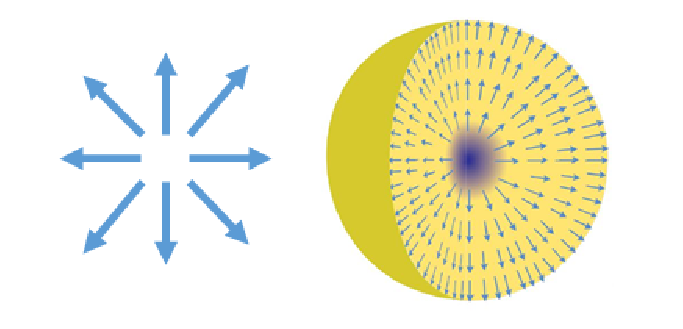
\includegraphics[width=\linewidth]{figures/defects.eps}
\caption{ The left picture is a vortex, which in two dimensions is a point topological defect. The right is a hedgehog, which is a point topological defect in three dimensions.
\label{topo_defects}}
%\end{wrapfigure}
\end{wrapfigure}

The study of a bosonic TI was begun by Vishwanath and Senthil in 2013\cite{SenthilVishwanath}. They produced effective field theories for the bulk of the bosonic TI which are consistent with Eq.~(\ref{externEB}). One important different in the boson case is that for bosons the `integer quantum Hall effect' has a Hall conductivity quantized to even integers (see Section \ref{subsec::FQHEintro}). Therefore by the same arguments as for the fermionic case $\theta$ is $4\pi$-periodic, and therefore in the presence of time reversal symmetry $\theta$ is quantized to be either $0$ or $2\pi$. 

Ref.~\cite{SenthilVishwanath} also produced an effective field theory for the surface of the boson TI. As one would expect on the surface of a SRE topological phase, they found a number of different phenomena which cannot exist in a purely two-dimensional system, and can only exist on the surface of a topological phase. In the free fermionic topological insulator, the possible edge phases either are gapless (Dirac cones) or break one of the symmetries of the system (either charge conservation or time reversal). The system considered by Ref.~\cite{SenthilVishwanath} has no Dirac cones. In studies of the bosonic quantum Hall effect it is convenient to enlarge the charge conservation symmetry to $\uxu$ (two species of bosons). The surface effective field theory of Ref.~\cite{SenthilVishwanath} can produce exotic superfluid phases which break at least one of these symmetries, and it can also realize a time-reversal symmetry broken phase which has a Hall conductivity quantized to an odd integer (impossible in a purely two-dimensional boson system). Most interestingly, they also find a surface phase which is gapped and breaks none of the symmetries of the system, but which contains LRE topological order.

The effective field theory of Ref.~\cite{SenthilVishwanath} is a powerful tool for describing topological phases, but it does not tell us whether a microscopic model described by this effective theory exists, and it gives us little intuition into what properties such a microscopic model might have. To answer these questions, we have constructed a microscopic model which realizes the boson TI, and this work is the subject of Chapter \ref{chapter::SO34D}.
The model uses many of the same techniques as used to study the boson QHE in Chapter \ref{chapter::FQHE}. In the boson QHE case, we were working in two dimensions, and we realized the phase of interest by binding bosons to point topological defects (vortices), and condensing the resulting bound states. In the boson TI, we will again bind bosons to point topological defects and condense the bound states. In this case the point topological defects are called hedgehogs (see Fig.~\ref{topo_defects}). One way to model such hedgehogs is to introduce $SO(3)$ spins onto our lattice, and define a hedgehog as existing whenever the spins have a configuration like that in Fig.~\ref{topo_defects}. This method provides intuition for understanding our setup, but unfortunately it does not allows us to make quantitatively accurate measurements. Alternatively, we can introduce hedgehogs into our model by starting with a set of boson variables, and describing these bosons with a parton description. The redundancy of this description introduces an internal gauge field, and we can identify monopoles of this gauge field with the hedgehogs. By binding these hedgehogs to a second species of bosons, we produce the boson TI. This is also a nice description because it is a model of two species of bosons, like that in Ref.~\cite{SenthilVishwanath}. Both of these methods of representing the hedgehogs can be studied in sign-free Monte Carlo simulations.

We can make a number of measurements on our model to determine that it is in fact a boson TI. We can study the surface of the model, and like Ref.~\cite{SenthilVishwanath} we find exotic superfluids which break one of the $U(1)$ symmetries. By explicitly breaking the time-reversal symmetry we can put the system into a phase with a Hall conductivity, and by measuring this Hall conductivity (and finding a value not allowed in a purely two-dimensional system) we can convincingly argue that the bulk of our system is in a topological phase. We can also find a surface phase which is gapped and breaks no symmetries, and we argue that it is therefore the long-ranged entangled phase of Ref.~\cite{SenthilVishwanath}.

We can also measure the Witten effect, as described above for the fermionic TI and extended to the boson TI by Refs.~\cite{Max,MaxWitten}. In our system we study two species of bosons which are coupled to different external gauge fields. The Witten effect in this setup is the statement that a monopole of one of the gauge fields will have a half-integer charge bound to it of the boson species coupled to the other gauge field. If the two external gauge fields were identified, we would get an integer charge bound to each monopole, which is what is predicted by Eq.~(\ref{externEB}) with $\theta=2\pi$. We could cancel this integer charge by adding a boson to the monopole, but this would turn the monopole into a fermion, a manifestation of the `statistical Witten effect'\cite{Max,MaxWitten}.

Our models also allow us to bind multiple hedgehogs to each boson. We find that this leads to a model with gapped excitations that carry fractional charge, and therefore we call this the fractional topopological insulator of bosons, and it is an LRE topological phase. The model also contains gapped excitations which are quantum lines, and when a fractionally charged quasiparticle is exchanged with these lines the action is changed by an anyonic phase (i.e.~a phase not $0$ or $\pi$). We find that the surface of the fractional phase has a Hall conductivity quantized to a rational number (which is not possible without long-ranged entanglement), and it exhibits a Witten effect where one of the fractionally charged quasiparticles is bound to the magnetic monopole.

%%%%%%%%%%%%%%%%%%%%%%%%%%%%%%%%%%%%%%%%%%%%%%%%%%%%%%%%%%%%%%%%%%%%%%%%%%%%%%%%%%%5
\section{Topological Quantum Computing and Numerical Studies of the Quantum Hall Effect}

In recent decades, the field of quantum computing has been a very active field of physics research. The excitement in this field comes from the fact that, in general, the amount of time it takes to find the ground state of a quantum Hamiltonian scales exponentially in the size of the system. Yet nature manages to use quantum mechanics to solve such systems efficiently, and this raises the question of what other computationally hard problems can be solved by a quantum mechanical system, or `quantum computer'. Such quantum computers have many practical applications, such as their ability to factor large numbers. They are also exciting as an aid to condensed matter physicists, who could use them to find the ground states of model Hamiltonians.

Constructing such a quantum computer requires overcoming a large number of experimental challenges, perhaps the most daunting of which is the phenomena of decoherence. Imagine, for example, a quantum computer constructed out of a number of cold atoms, which have an internal degree of freedom which we can model as a spin-1/2. The spin-1/2's form the `qubits', and the states of the quantum computer are all wavefunctions of these spins. If we work in, for example, the $z$ basis, a wavefunction is a linear superposition of a number of $z$-eigenstates, each of which has some spins pointing up and others down. Local perturbations can change the state of the computer either by flipping a spin or by changing the relative phases of the different eigenstates (these are called phase errors). This phenomenon is called decoherence, and it means that any information stored on a quantum computer will quickly be lost.

The problem of decoherence exists in classical computers as well, but it is somewhat simpler in that the only error is the flip of a bit. In this case `error-correcting codes' can be used to redundantly store information. These error correcting codes can make classical computers essentially error-free. Error-correcting codes exist for quantum systems as well, but in a quantum computer there are more ways for errors to happen, in particular phase errors. This means that quantum error-correcting codes must be more complicated, and in practice hundreds to thousands of spin-1/2's are needed to create a single error-protected qubit. Constructing a quantum computer with such a large number of physical degrees of freedom is an extremely difficult task.

One way to avoid this problem is by constructing a `topological quantum computer out' of long-ranged entangled topological phases. The reason this may work is because such phases have degenerate ground states. We can let the state of the quantum computer be described by which degenerate ground state the system is in. The important observation is that in order to connect degenerate ground states in, for example, a fractional quantum Hall system on a torus, a quasiparticle must be brought all the way around a cycle of the torus. The probably of this happening by purely local perturbations scales as $e^{-L}$, where $L$ is the linear dimension of the system. This is very small in the thermodynamic limit, and so local perturbations cannot change the state of the computer and the system is immune to decoherence.

The fractionalized quasiparticles (`anyons') in the fractional quantum Hall effect can store quantum information in way which is robust against decoherence, but they cannot perform all the computations on this information needed to build a true quantum computer. This is because they are Abelian, which means that the operations of exchanging them commute, it only changes the wave function by a phase. To build a `universal' quantum computer one needs more exotic quasiparticles known as non-Abelian anyons. Exchanging two of these quasiparticles changes the ground state of the system, with the number of ground states given by $d^N$, where $N$ is the number of non-Abelian anyons and $d$ is the `quantum dimension' of the anyons. 

Theoretically, there are a number of different types of non-Abelian anyons. The simplest and best-known is the Majorana fermion. Though the Majorana fermion cannot be used for universal quantum computation, it can still interesting for its applications to long-lived quantum memory\cite{KitaevWireMajorana:01}, as well as for its unique physical properties. Techniques developed by realizing Majorana fermions experimentally may also be useful for realizing its more complicated relatives. The Majorana fermion is also called a `$\ztwo$ parafermion', because combining two of them gives something Abelian. This can be generalized to $\mathbb{Z}_k$ parafermions, for integer $k$. For $k\ge 4$ these can be used for universal quantum computation\cite{CuiWang}. Another anyon which can be used for universal quantum computation is the Fibonacci anyon.

Since these non-Abelian anyons can be used for universal and fault-tolerant quantum computation, they being actively sought-after experimentally. Many experimental proposals involve constructing heterostructures of phases such as superconductors, topological insulators, ferromagnets, and wires with strong spin-orbit coupling\cite{AliceaReview}. Most of these proposals are for realizing Majorana fermions, and some proposals have been carried out possible detection of Majorana fermions\cite{MourikZuo:InSbWire:2012,Nadj-PergeYazdani:2014}. Experiments for realizing other anyons in heterostructures have also been proposed\cite{SOCALBS}.

Another approach would be to find long-ranged entangled topological phases which have non-Abelian anyons as their gapped quasiparticles. In particular, Moore and Read\cite{MooreRead} proposed that the quantum Hall effect at $\nu=5/2$ can host Majorana fermions. Non-Abelian phases which can exist at other filling fractions have been proposed as well\cite{Read-PhysRevB.59.8084,BondersonSlingerland}. Unfortunately, even if a given non-Abelian phase is consistent with a given filling fraction, this does not mean that that non-Abelian phase is the ground state for the systems prepared at that filling by experimentalists. 

It is therefore an important problem to determine whether the quantum Hall states realized experimentally are indeed the sought after non-Abelian phases. This may be possible experimentally, but as the experiments are likely very difficult it is up to theorists to provide guidance as to which filling fractions are most likely to host non-Abelian phases, and under what conditions. Unfortunately, performing this task requires quantitatively estimating the energy of the possible ground states in the strongly interacting quantum Hall problem, and this is very difficult analytically.

In order to determine whether the non-Abelian phase is indeed the ground state of a realistic system we therefore turn to numerics. Particularly, these systems can be studied using density matrix renormalization group (DMRG) algorithms\cite{ZaletelQHdmrg13, ZaletelMixing}. DMRG is a variational method which works well for one-dimensional, gapped systems. To study a quantum Hall system, we put the system on a cylinder. The computing resources required to study the system scale as $e^L$, with $L$ the circumference of the cylinder. Though this exponential growth is unfortunate, it is in only one of the two dimensions of the system, and this compares well with the rival method, exact diagonalization, which scales as $e^{L^2}$. 

A promising place to look for non-Abelian quantum Hall phases is in quantum Hall bilayers: systems composed of two quantum wells, each of which hosts a quantum Hall effect. Such bilayers have been studied experimentally, primarily at fillings $1/2+1/2$ (each layer is at $\nu=1/2$) and $1/4+1/4$\cite{JimReview}. One advantage to studying these bilayers is their tunability: experimentalists can change the distance between the two layers as well as the tunneling between the layers, and this can tune the system between different quantum Hall phases. One can hope that we can experimentally tune the bilayer system into a phase which hosts non-Abelian anyons.

In Chapter \ref{chapter::bilayer} I describe an DMRG study of a bilayer system at filling $1/3+1/3$. We obtain the phase diagram in terms of the tunable parameters of layer separation and interlayer tunnelling, and also investigate the effects of finite layer width. We find transitions between a number of different Abelian phases, and we investigate the nature of these phase transitions. All of these phases have the same symmetry (there is no local order parameter which can distinguish them) and the same Hall conductivity, but we identify the phases using other properties related to their entanglement structure.

The phases which we find by modifying the experimentally tunable parameters are all Abelian. To find phases which host non-Abelian anyons we further modify the Coulomb interaction. Experimentally there are number of ways to modify the Coulomb interaction, such as studying higher Landau levels, allowing mixing between the Landau levels, or changing the shape of the quantum wells. We find that by reducing the repulsion between electrons in different layers, we are able to tune the system into a non-Abelian phase. We measure a number of properties of this phase, and determine that it is a phase called the `interlayer Pfaffian', which hosts a Majorana fermion.


%DMRG methods have already been applied to look for non-Abelian phases in quantum Hall systems at $\nu=5/2$ and $\nu=12/5$. In Chapter \ref{chapter::bilayer} I discuss an application of this procedure for a bilayer quantum Hall system, where each layer has $\nu=1/3$. One advantage of studying bilayer systems is that the experimentally there are more ways to tune the interactions in the system. By using DMRG on a realistic Hamiltonian we found the phase diagram of the system in the experiment


%I was able to determine that the most straightforward experiment will not see any non-Abelian phases. I was however able to address other experimentally relevant questions such as the nature of the Abelian topological phases expected, the order of the transitions between them, the effects of having quantum wells of finite width, and the magnetic field needed to spin polarize the system.

%In addition, I was able to determine what changes to the Coulomb interaction between electrons would lead to a non-Abelian phase, and identify the resulting non-Abelian phase as the `interlayer Pfaffian'.

\section{Overview of contributions}

Figure \ref{papers} shows a representation of all of the publications produced during my graduate research. Not all of the publications in this figure will be adequately covered in this report, this figure has been included to show how the projects that I will discuss fit into the other research that I have done. 

\begin{wrapfigure}{r}{0.5\textwidth}
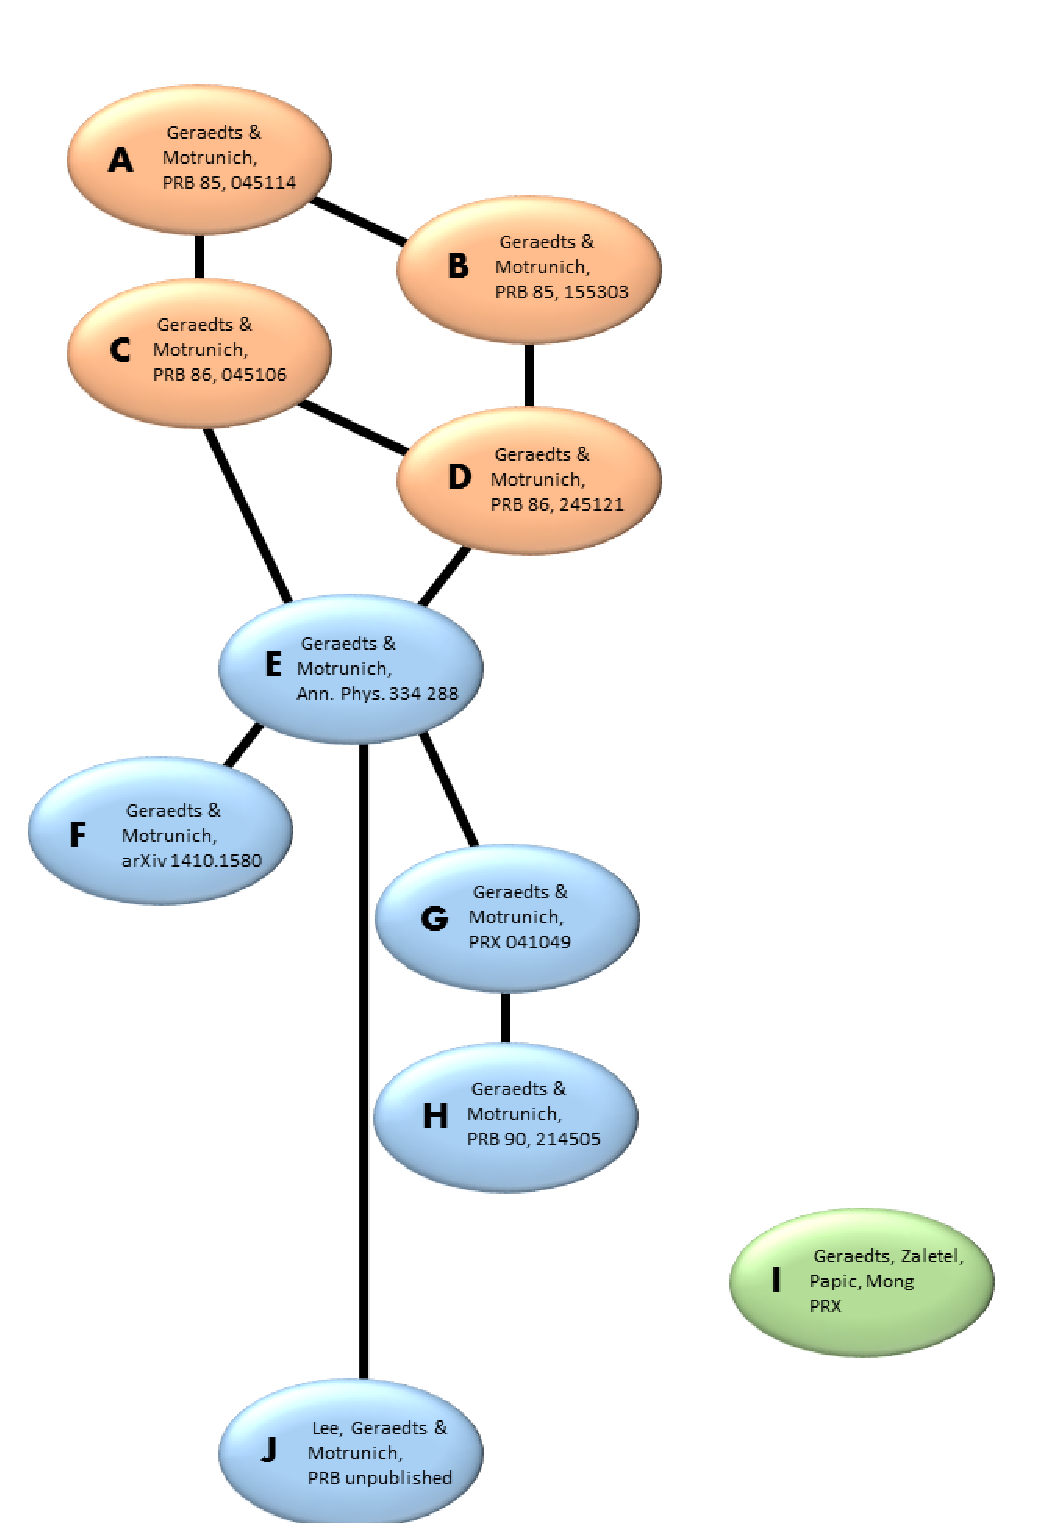
\includegraphics[width=\linewidth]{figures/publications.eps}
\caption{ An overview of all the papers discussed in this work. The vertical direction is time, and black arrows mean that results of one paper were used in the next. Details for the various figures are described in the text.
\label{papers}}
\end{wrapfigure}

The papers are divided into three categories: orange, blue and green. The orange category contains work done to develop the statistical mechanics models of bosons with mutual statistics. The paper marked A \cite{Loopy} in the figure was the first to study such models in sign-free Monte Carlo simulations. It was specialized to the case where the bosons were mutual fermions, and interacted with each other on-site interactions. 
The paper marked B\cite{Ranged_Loops} was a related study of a system with only a single species of bosons, but these bosons had `marginally long-ranged' ($1/r^2$) interactions. The order of the Mott insulator-superfluid transition in this system was the subject of some controversy, and we definitively showed that the transition was second order while also developing the numerical techniques needed to handle bosons with arbitrary interactions. 
Paper C\cite{short_range3} also studied bosons with delta function interactions but generalized the mutual statistics of the two species to be any number. (The bosons were `mutual anyons', instead of `mutual fermions') 
Finally paper D\cite{Gen2Loops} generalized our methods to any interaction and any mutual statistics. In particular we focussed on the marginally-long-ranged case, where our analytical tools allowed for the complete establishment of the phase diagram. The results found for the various models studied in these papers will not be discussed in this report. However, the methods used to study these systems proved extremely useful throughout my graduate research, and so these methods are outlined in Chapter \ref{chapter::methods}. Also, the results of paper C are featured in Section \ref{sec:reverse}, where they are used to understand the phase diagram of bosonic quantum Hall phases.

The blue category takes the methods developed in the orange category and applies them to the problem of studying topological phases of bosons. In Paper E\cite{FQHE}, which is discussed in Chapter \ref{chapter::FQHE}, the method are applied to the bosonic topological insulator. We next wanted to apply the same methods to three-dimensional topological phases. To gain some intuition for this we first went backward and developed an exactly solvable model for a class of one-dimensional topological phases, which is described in paper F\cite{1DSPT}. In Paper G\cite{SO34D}, which is discussed in Chapter \ref{chapter::SO34D}, we successfully construct a model for the three-dimensional bosonic topological insulator. In paper H\cite{FracFaraday} we consider a variant of our model for the boson fractional topological insulator, which instead realizes a novel long-range entangled phase of a lattice gauge theory. Finally in paper J\cite{JongYeon} we use the model of the boson QHE to study the transitions between different quantum Hall phases. All of the above work was done in collaboration with Lesik Motrunich.

The green category covers the work on the (fermionic) fractional quantum Hall effect accomplished using DMRG. This category contains only paper I\cite{bilayer}, and is discussed in Chapter \ref{chapter::bilayer} This work was done in collaboration with Roger Mong, Mike Zaletel and Zlatko Papic.
